\documentclass[11pt]{article}
\usepackage{amsmath, amsthm, amssymb, pdfpages} 
\usepackage{fullpage}
\usepackage{hyperref}
\usepackage{graphicx}
\usepackage[capitalize]{cleveref}

% next three for UTF8 to work (for non-ASCII names to work without awkward codes)
\usepackage[T1]{fontenc}
\usepackage{textcomp}
\usepackage[utf8]{inputenc}

% import biblatex with prefered settings
% reuse code and library from RGLS paper in the same repository
% loads biblatex with all the nice standard options that John determined some time ago!
% this version uses a ``Harvard'' style (first author last name, year in parentheses).
% also loads xpatch

% biblatex
% harvard style
\usepackage[style=authoryear,natbib,maxcitenames=2,doi=false,isbn=false,url=false,backend=bibtex]{biblatex}
% numeric style
%% \usepackage[style=numeric-comp,sorting=none,giveninits=true,
%%                      doi=false,isbn=false,url=false,backend=bibtex]{biblatex}
% remove "In: " before journal title
\renewbibmacro{in:}{}
% remove language
\AtEveryBibitem{\clearlist{language}}
% remove month
\AtEveryBibitem{\clearfield{month}}
% and also notes
\AtEveryBibitem{\clearfield{note}}
% remove dots between volume and issue
\usepackage{xpatch}
\xpatchbibmacro{volume+number+eid}{%
  \setunit*{\adddot}%
}{%
}{}{}
% put issue in parentheses
\DeclareFieldFormat[article]{number}{\mkbibparens{#1}}


\bibliography{../manuscripts/zotero, ../manuscripts/dummy} % biblatex wants this in the preamble...

% define shortcuts for awkward math symbols
% this also helps us change them more easily later, if needed
\newcommand{\rmsd}{\text{RMSD}_p}
\newcommand{\auc}{\text{AUC}_\text{PR}}

\usepackage[noT]{kinshipsymbols}
% % copy of \Fst from package `kinshipsymbols`
%\newcommand{\Fst}{F_\text{ST}}

% double line spacing (PLoS wants this)
\usepackage{setspace}
\doublespacing
% original, smaller spacing
%\renewcommand{\baselinestretch}{1.2}

\title{\Large \textbf{Testing the effectiveness of principal components in adjusting for relatedness in genetic association studies}}
\author{Yiqi Yao$^1$, Alejandro Ochoa$^{1,2,*}$}
\date{}

\begin{document}
\maketitle

\noindent
$^1$ Department of Biostatistics and Bioinformatics, Duke University, Durham, NC 27705, USA \\
$^2$ Duke Center for Statistical Genetics and Genomics, Duke University, Durham, NC 27705, USA \\
$^*$ Corresponding author: \texttt{alejandro.ochoa@duke.edu}


\begin{abstract}
  Modern genetic association studies require modeling population structure and family relatedness in order to calculate correct statistics.
  Principal Components Analysis (PCA) is one of the most common approaches for modeling this population structure, but nowadays the Linear Mixed-Effects Model (LMM) is believed by many to be a superior model.
  Remarkably, previous comparisons have been limited by testing PCA without varying the number of principal components (PCs), by simulating unrealistically simple population structures, and by not always measuring both type-I error control and predictive power.
  In this work, we thoroughly evaluate both PCA and LMMs with varying number of PCs in various realistic scenarios, including admixture together with family structure, measuring both null p-value uniformity and the area under the precision-recall curves.
  We find that LMM without PCs performs best overall, although PCA performs as well as LMM when enough PCs are used, there are no close relatives, and the sample size is large.
  We also find a remarkable robustness to extreme numbers of PCs.
  Altogether, we recommend LMMs in general for association studies, but find that PCA performs as well as LMMs in many common scenarios.
\end{abstract}

% \clearpage

% \tableofcontents

\clearpage
	
\section{Introduction} 

The goal of a genetic association study is to identify loci whose genotypes are correlated significantly with a certain trait.
An important assumption made by classical association tests is that genotypes are unstructured: drawn independently from a common allele frequency.
However, this assumption does not hold for structured populations, which includes multiethnic cohorts and admixed individuals, and for family data.
When naive approaches are incorrectly applied to structured populations and/or family data, association statistics (such as $\chi^2$) become inflated relative to the null expectation, resulting in greater numbers of false positives than expected and loss of power \citep{devlin_genomic_1999, voight_confounding_2005, astle_population_2009}.

The most popular approaches for conducting genetic association studies with structured populations involve modeling the population structure via covariates.
Such covariates may be inferred ancestry proportions \citep{pritchard_association_2000} or transformations of these.
Principal components analysis (PCA) represents the most common of these variants, in which the top eigenvectors of the kinship matrix are used to model the population structure \citep{zhang_semiparametric_2003, price_principal_2006, bouaziz_accounting_2011}.
These top eigenvectors are commonly referred to as Principal Components (PCs) in the genetics literature (the convention we adopt here; \cite{patterson_population_2006}), but it is worth noting that in other fields the PCs would instead denote the projections of the data onto the eigenvectors \citep{jolliffe_principal_2002}.
Various works have found that PCs map to ancestry, and PCs work as well as ancestry in association studies and can be inferred more quickly \citep{patterson_population_2006, zhao_arabidopsis_2007, bouaziz_accounting_2011}.
More recent work has focused on speeding up the calculation of PCs rather than on evaluating its performance in association studies \citep{lee_sparse_2012, abraham_fast_2014, galinsky_fast_2016, abraham_flashpca2:_2017}.
PCA remains a popular and powerful approach for association studies \citep{wojcik_genetic_2019}.

The other dominant approach for genetic association studies under population structure is the Linear Mixed-effect Model (LMM), in which population structure is a random effect drawn from a covariance model parametrized by the kinship matrix.
LMM and PCA share deep connections that suggest that both models ought to perform similarly \citep{astle_population_2009, janss_inferences_2012, hoffman_correcting_2013}.
However, many previous studies have found that LMM outperforms the PCA approach, although many evaluations have been limited \citep{zhao_arabidopsis_2007, astle_population_2009, kang_variance_2010}.
Other studies find that PCA can outperform LMM in certain settings \citep{price_new_2010, wu_comparison_2011, wang_analytical_2013}, although these are believed to be unusual \citep{sul_mixed_2013}.
Moreover, various explanations for if and why LMM outperforms PCA are vague and have not been tested directly \citep{price_new_2010, sul_mixed_2013, price_response_2013, hoffman_correcting_2013}.
Since LMMs tend to be considerably slower than the PCA approach, it is important to understand when the difference in performance between these two approaches is outweighed by their difference in runtime.

PCA has been evaluated in numerous previous works in the context of association studies.
However, all of these studies have important limitations, for the most part due to PCA being treated as a competitor rather than a method worthy of exploring more fully.
For example, although there are methods for selecting the numbers of PCs \citep{patterson_population_2006}, most evaluations either admit to selecting 10 because it has long been the default and it performs well enough, regardless of the dataset in question \citep{epstein_simple_2007, li_improved_2008, astle_population_2009, li_correcting_2010, wu_comparison_2011}, or test only one number of PCs without much justification \citep{zhang_semiparametric_2003, kimmel_randomization_2007, zhao_arabidopsis_2007, zhang_comparison_2008, price_new_2010, bouaziz_accounting_2011, hoffman_correcting_2013, wang_analytical_2013, tucker_improving_2014, yang_advantages_2014, sul_population_2018}.
Conversely, only a few studies consider a (small) set of numbers of PCs, where they show remarkable robustness to this choice \citep{price_principal_2006, kang_variance_2010, wojcik_genetic_2019}.
Moreover, most of these evaluations considered simulated data with only $K = 2$ independent subpopulations or admixture from only two subpopulations (exceptions are \citet{astle_population_2009} with $K=3$, and \citet{wang_analytical_2013} with $K = 4$), although worldwide human population structure is expected to have a larger dimensionality of at least $K = 9$ \citep{wojcik_genetic_2019}.
Similarly, only one evaluation simulated data from a family pedigree: \citet{price_new_2010} included sibling pairs.
Some studies include evaluations involving real data that featured known or cryptic relatedness, but these analyses did not measure type-I error rates or power calculations, most of which settled for measuring test statistic inflation.
Lastly, many of the earlier evaluations employed case-control simulations exclusively (as opposed to quantitative traits as we do here), were based on very small real or simulated datasets relative to today's standards, did not include any LMMs in their evaluations, and often did not measure both type-I error rates and power (or one of their proxies).
Here we aim to systematically evaluate the robustness of both the PCA (fixed effects only) and LMM (mixed effects) approaches to the choice of number of PCs, especially in cases where the model is grossly misspecified, in more realistic simulations relevant to today's genetics research.

In this work, we study the performance of the PCA and LMM methods in genetic association studies, characterizing their behavior under various numbers of PCs (for LMM as well as PCA) and varying sample sizes, under a reasonable admixture model with $K = 10$ source subpopulations and also a model with admixture and family structure.
Our evaluation is more thorough than previous ones, directly measuring the uniformity of null p-values (as required for accurate type-I error control and FDR control via q-values; \cite{storey_positive_2003, storey_statistical_2003}) and predictive power by calculating the area under precision-recall curves.
Across all tests we find that LMM without PCs performs best, but PCA matches that optimal performance when sample sizes are large (at least 1,000 individuals) and there are no close relatives in the study.
Remarkably, PCA is robust even when the number of PCs far exceeds the optimal number for reasonably large studies.
However, for smaller studies (100 individuals) there is a more pronounced loss of power for PCA when the number of PCs exceeds the optimal number.
LMMs significantly outperforms PCA in the presence of family structure, which is a well-known case where PCA fails \citep{patterson_population_2006, price_new_2010}.
We also found that LMM without PCs always outperforms use of any number of PCs in the LMM.
All together, our simulation studies indicate that LMMs are preferable, and provide clear criteria under which use of PCA results in acceptable performance compared to LMMs.

% TODO Missing:
% \begin{itemize}
% \item Proposed simulation to infer optimal number of PCs from real data, predict gap between PCA and LMM?
% \item Small sample size GCTA should change NAs to something bad (0 AUC, but what RMSD?)
% \item Add independent subpopulations (what Yiqi originally had) alongside for clear higher $r$ cases
% \item Plot of kinship matrices of each simulation (more useful when Indep Subpops are added)
% \item Selection simulation
% \item Rare variant simulation
% \end{itemize}

\section{Models and Methods}

\subsection{Models for genetic association studies}

In this subsection we describe the complex trait model and kinship model that motivates both the PCA and LMM models for genetic association studies, followed by further details regarding the PCA and LMM approaches.
The derivations of the PCA and LMM models from the general quantitative trait model are similar to previous presentations \citep{astle_population_2009, janss_inferences_2012, hoffman_correcting_2013}, but we emphasize the kinship model for random genotypes as being crucial for these connections, and make a clear distinction between the true kinship matrix and its most common estimator, which is biased \citep{ochoa_fst2, ochoa_human}.

\subsubsection{The complex trait model and PCA approximation}

Let $\xij \in \{ 0, 1, 2 \}$ be the genotype at locus $i$ for individual $j$, which counts the number of reference alleles.
Suppose there are $n$ individuals and $m$ loci,
$\mathbf{X} = ( \xij )$ is their $m \times n$ genotype matrix, and
$\mathbf{y}$ is the length-$n$ (column) vector which represents trait value for each individual.
The approaches we consider are based on the following additive linear model for a quantitative (continuous) trait:
\begin{equation}
  \label{eq:trait}
  \mathbf{y}
  =
  \mathbf{1} \alpha + \mathbf{X}^\intercal \mathbf{\beta} + \mathbf{\epsilon}
  ,
\end{equation}
where
$\mathbf{1}$ is a length-$n$ vector of ones,
$\alpha$ is the scalar intercept coefficient,
$\mathbf{\beta}$ is the length-$m$ vector of locus effect sizes, and
$\mathbf{\epsilon}$ is a length-$n$ vector of residuals.
The residuals are assumed to follow a normal distribution: $\mathbf{\epsilon}_j \sim \text{Normal}(0, \sigma^2)$ independently for each individual $j$, for some residual variance parameter $\sigma^2$.

Typically the number of loci $m$ is in the order of millions while the number of individuals $n$ is in the thousands.
Hence, the full model above cannot be fit in this typical $n \ll m$ case, as there are only $n$ datapoints to fit (the trait vector) but there are $m+1$ parameters to fit ($\alpha$ and the $\mathbf{\beta}$ vector).
The PCA model with $r$ PCs approximates the full model fit at a single locus $i$:
\begin{equation}
  \label{eq:pca_gwas}
  \mathbf{y}
  =
  \mathbf{1} \alpha + \mathbf{x}_i \beta_i + \mathbf{U}_r \mathbf{\gamma}_r + \mathbf{\epsilon}
  ,
\end{equation}
where $\mathbf{x}_i$ is the length-$n$ vector of genotypes at locus $i$ only,
$\beta_i$ is the effect size coefficient for that locus,
$\mathbf{U}_r$ is an $n \times r$ matrix of PCs, and
$\mathbf{\gamma}_r$ is the length-$r$ vector of coefficients for the PCs.
This approximation is explained by first noticing that the genotype matrix has the following singular value decomposition:
$\mathbf{X}^\intercal = \mathbf{U} \mathbf{D} \mathbf{V}^\intercal$,
where assuming $n < m$ we have that
$\mathbf{U}$ is an $n \times n$ matrix of the left singular vectors of $\mathbf{X}$,
$\mathbf{V}$ is an $m \times n$ matrix of its right singular vectors, and
$\mathbf{D}$ is an $n \times n$ diagonal matrix of its singular values.
Thus, in the full model we have
$\mathbf{X}^\intercal \mathbf{\beta} = \mathbf{U} \mathbf{\gamma}$,
where
$\mathbf{\gamma} = \mathbf{D} \mathbf{V}^\intercal \mathbf{\beta}$ is a length-$n$ vector.
The approximation consists solely of replacing $\mathbf{U} \mathbf{\gamma}$ (the full set of $n$ left singular vectors and their coefficients) with $\mathbf{U}_r \mathbf{\gamma}_r$ (the top $r$ singular vectors only, which constitutes the best approximation of rank $r$).
Thus, the extra terms in the PCA approach approximate the polygenic effect of the whole genome, and assumes that the locus $i$ being tested does not contribute greatly to this signal.

The statistical significance of a given association test is performed as follows.
The null hypothesis is $\beta_j = 0$ (no association).
The null and alternative models are each fit (fitting the coefficients of the multiple regression, where $\beta_j$ is excluded under the null while it is fit under the alternative).
The resulting regression residuals are compared to each other using the F-test, which results in a two-sided p-value.
Note that many common PCA implementations trade the more exact F-test for a $\chi^2$ test, which is simpler to implement but only asymptotically accurate.
As this is a multiple hypothesis test, there are a large number of loci ($m$) tested for association, so it is best to control the FDR rather than setting a fixed p-value threshold.
We recommend estimating q-values and setting a threshold of $q < 0.05$ so that the FDR is controlled at the 5\% level.

\subsubsection{Kinship model for genotypes}

In order to better motivate the most common estimation procedure of PCs for genotype data, and to connect PCA to LMMs, we shall review the kinship model for genotypes.
The model states that genotypes are random variables with a mean and covariance structure given by
$$
\E[ \xij ]
=
2 \pit,
\quad\quad
\Cov( \xij, \xij[k] )
=
4 \pit ( 1 - \pit ) \kt,
$$
where \pit is the ancestral allele frequency at locus $i$ and \kt is the kinship coefficient between individuals $j$ and $k$ \citep{malecot_mathematiques_1948, wright_genetical_1951, jacquard_structures_1970}.
Thus, if we standardize the genotype matrix as
$$
\mathbf{X}_S
=
\left(
  \frac{
    \xij - 2 \pit
  }{
    \sqrt{4 \pit \left( 1 - \pit \right)}
  }
\right)
,
$$
then this results in a straightforward kinship matrix estimator:
$$
\E
\left[
\frac{1}{m}
\mathbf{X}_S^\intercal
\mathbf{X}_S
\right]
=
\mathbf{\Phi}
,
$$
where $\mathbf{\Phi} = ( \kt )$ is the $n \times n$ kinship matrix.
Note that replacing the raw genotype matrix $\mathbf{X}$ with the standardized matrix $\mathbf{X}_S$ in the trait model of \cref{eq:trait} results in an equivalent model, as this covariate differs only by a linear transformation.
Thus, under the standardized genotype model, the PCs of interest are equal in expectation to the top eigenvectors of the kinship matrix.

\subsubsection{Estimation of principal components from genotype data}

In practice, the matrix of principal components $\mathbf{U}_r$ in \cref{eq:pca_gwas} is determined from an estimate of the earlier standardized genotype matrix $\mathbf{X}_S$, namely
$$
\mathbf{\hat{X}}_S
=
\left(
  \frac{
    \xij - 2 \pith
  }{
    \sqrt{4 \pith \left( 1 - \pith \right)}
  }
\right)
,
$$
where the true ancestral allele frequency \pit is replaced by the estimate
$
\pith = \frac{1}{2n} \sum_{j = 1}^n \xij,
$
and results in the kinship estimate
$
\mathbf{\hat{\Phi}}
=
\frac{1}{m}
\mathbf{\hat{X}}_S^\intercal
\mathbf{\hat{X}}_S
.
$
This kinship estimate and minor variants are also employed in LMMs \citep{yang_gcta:_2011}.
This estimator of the kinship matrix is biased, and this bias is different for every individual pair \citep{ochoa_fst2, ochoa_human}.
However, in the present context of PCA regression in genetic association studies, the existing approach performs as well as when the above estimate is replaced by the true kinship matrix (not shown).
Thus, it appears that in combination with the intercept term ($\mathbf{1} \alpha$ in \cref{eq:pca_gwas}), the rowspace of this kinship matrix estimate approximately equals that of the true kinship matrix.

\subsubsection{Linear mixed-effects model}

The LMM is another approximation to the complex trait model in \cref{eq:trait}.
Excluding additional covariates first, the LMM is
\begin{equation}
  \label{eq:lmm_gwas}
  \mathbf{y}
  =
  \mathbf{1} \alpha + \mathbf{x}_i \beta_i + \mathbf{s} + \mathbf{\epsilon}
  ,
\end{equation}
which is like the PCA model in \cref{eq:pca_gwas} except that the PC terms $\mathbf{U}_r \mathbf{\gamma}_r$ are replaced by the random effect $\mathbf{s}$, which is a length-$n$ vector drawn from
$$
\mathbf{s} \sim \text{Normal} \left( \mathbf{0}, \sigma^2_s \mathbf{\Phi} \right),
$$
where $\mathbf{\Phi}$ is the kinship matrix and $\sigma^2_s$ is a trait-specific variance scaling factor.
This model is derived from treating the standardized genotype matrix $\mathbf{X}_S$ as random rather than fixed, so that the standardized genetic effect
$\mathbf{X}_S^\intercal \mathbf{\beta}_S$
in \cref{eq:trait} has mean zero and a covariance matrix of
$$
\Cov \left( \mathbf{X}_S^\intercal \mathbf{\beta}_S \right)
=
|| \mathbf{\beta}_S ||^2 \mathbf{\Phi}
.
$$
The above random effect $\mathbf{s}$ satisfies those equations, where the variance scale equals $\sigma^2_s = || \mathbf{\beta}_S ||^2$.
Thus, the PCA approach is the fixed model equivalent of the LMM under the additional approximation that only the top $r$ eigenvectors are used in PCA whereas the LMM uses all eigenvectors.

A key advantage of LMM over PCA is that it has fewer parameters to fit: ignoring the shared terms in \cref{eq:pca_gwas} and \cref{eq:lmm_gwas}, PCA has $r$ parameters to fit (each PC coefficient in the $\mathbf{\gamma}$ vector), whereas LMMs only fit one additional parameter, namely $\sigma^2_s$.
Therefore, PCA is expected to overfit more substantially than LMM---and thus lose power---when $r$ is very large, and especially when the sample size (the number of individuals $n$) is very small.

Due to its accuracy and speed, the LMM implementation that we chose for our evaluations is GCTA \citep{yang_gcta:_2011}.
GCTA uses the same biased kinship matrix estimator $\mathbf{\hat{\Phi}}$ as standard PCA approaches, and the version that incorporates PCs also derives the PCs from the same kinship matrix estimate; thus, when both kinship and PCs are used, the population structure is essentially modeled twice, although some previous work has found this apparent redundancy beneficial \citep{zhao_arabidopsis_2007, price_new_2010}.
It is worth noting that earlier LMM approaches estimated kinship matrices using maximum likelihood approaches that excluded population structure from their estimates, and population structure was modeled via admixture proportions rather than PCA \citep{yu_unified_2006, zhao_arabidopsis_2007}.
When testing LMM with PCs, we use GCTA to estimate the PCs, which are included in GCTA as fixed effect covariantes.
Statistical significance in GCTA (and most other LMMs) is calculated via a likelihood ratio test, in which the test statistic has an asymptotic $\chi^2$ distribution under the null.

When running GCTA with large numbers of PCs in the small sample size particular simulation, we often encountered errors such as ``the information matrix is not invertible'', ``analysis stopped because more than half of the variance components are constrained'', and ``Log-likelihood not converged (stop after 100 iteractions)'' (sic), which make sense as we are pushing this complex model hard to be underconstrained, in which cases $\rmsd$ and $\auc$ were treated as missing.
These errors were not observed in our other simulations.


\subsection{Simulations}

\subsubsection{Genotype simulation from the admixture model}

We consider three simulation scenarios, refered to as (1) large sample size, (2) small sample size, and (3) family structure.
All cases are based on the admixture model described previously \citep{ochoa_fst1, ochoa_fst2}, and which is implemented in the R package \texttt{bnpsd} available on GitHub and the Comprehensive R Archive Network (CRAN).

Here we consider scenarios where the number of individuals $n$ varies:
the large sample size and family structure scenarios have $n = 1,000$ whereas small sample size has $n = 100$.
The number of loci in all cases is $m = 100,000$.
Individuals are admixed from $K = 10$ intermediate subpopulations, where $K$ is also the rank of the population structure; thus, after taking into account the intercept's rank-1 contribution, the population structure can be fit with $r = K-1$ PCs.
Each subpopulation $S_u$ ($u \in \{ 1, ..., K \}$) has an inbreeding coefficient $\ft[S_u] = u \tau$, individual-specific admixture proportions $q_{ju}$ for individual $j$ and intermediate subpopulation $S_u$ arise from a random walk model for the intermediate subpopulations on a 1-dimensional geography with spread $\sigma$, where the free parameters $\tau$ and $\sigma$ are fit to result in $\Fst = 0.1$ for the admixed individuals and a bias coefficient of $s = 0.5$, exactly as before \citep{ochoa_fst2}.

Random genotypes are drawn from this model, as follows.
First, uniform ancestral allele frequencies \pit are drawn.
The allele frequency $p_i^{S_u}$ at locus $i$ of each intermediate subpopulation $S_u$ is drawn from the Beta distribution with mean \pit and variance $\pit(1-\pit) \ft[S_u]$ \citep{balding_method_1995}.
The individual-specific allele frequency of individual $j$ and locus $i$ is given by
$
\pi_{ij} = \sum_{u = 1}^K q_{ju} p_i^{S_u}.
$
Lastly, genotypes are drawn from $\xij \sim \text{Binomial}(2, \pi_{ij})$.
Loci that are fixed (where for some $i$ we had $\xij = 0$ for all $j$, or $\xij = 2$ for all $j$) are drawn again from the model, starting from \pit, iterating until no loci are fixed.

\subsubsection{Genotype simulation from the family model}

Here we describe a simulation of a family structure with admixture that aims to be realistic by:
(1) pairing all individuals in every generation, resulting in two children per couple;
(2) strictly avoiding close relatives when pairing individuals;
(3) strongly favoring pairs that are nearby in their 1-dimensional geography, which helps preserve the population structure across the generations by preferentially pairing individuals with more similar admixture proportions (a form of assortative mating); and
(4) iterating for many generations so that a broad distribution of close and distant relatives is present in the data.

Generation 1 has individuals with genotypes drawn from the large sample size scenario described earlier, which features admixture.
In subsequent generations, every individual is paired as follows.
The local kinship matrix of individuals is stored and updated after every generation, which records the pedigree relatedness; in the first generation, everybody is locally unrelated.
Also, individuals are ordered, initially by the 1-dimensional geography, and in subsequent generations paired individuals are grouped and reordered by their average coordinate, preserving the original order when there are ties.
For every remaining unpaired individual, one is drawn randomly from the population, and it is paired with the nearest individual that is not a second cousin or closer relative (local kinship must be $< 1/4^3$).
Note that every individual is initially genderless, and after pairing one individual in the pair may be set to male and the other to female without giving rise to contradictions.
If there are individuals that could not be paired (occurs if unpaired individuals are all close relatives), then the process of pairing individuals randomly is repeated entirely for this generation.
If after 100 iterations no solution could be found randomly (there were always unpaired individuals), then the simulation restarts from the very first generation; this may occur for very small populations, but was not observed when $n = 1000$.
Once individuals are paired, two children per pair have their genotypes drawn independently of each other.
In particular, at every locus, one allele is drawn randomly from one of the parents and the other allele from the other parent.
Loci are constructed independently of the rest (no linkage disequilibrium).
The simulation continues for 20 generations.
As this simulation is very computationally expensive, it was run only once (genotypes did not change as new random traits were constructed as described next).

\subsubsection{Trait Simulation}

For a given genotype matrix (simulated or real), a simulated complex trait that follows the additive quantitative trait model in \cref{eq:trait} is constructed as follows.
In all cases we set the heritability of the trait to be $h^2 = 0.8$.
We varied the number of causal loci ($m_1$) together with the number of individuals ($n$) so power would remain balanced:
for the $n = 1,000$ cases we set $m_1 = 100$, whereas the $n = 100$ simulation had $m_1 = 10$.

Each simulation replicate consists of different causal loci with different effect sizes, as follows.
The non-genetic effects are drawn from $\epsilon_j \sim \text{Normal}(0, 1 - h^2 )$ independently for each individual $j$.
A subset of size $m_1$ of loci was selected at random from the genotype matrix to be causal loci.
The effect size $\beta_i$ at each causal locus $i$ is drawn initially from a Standard Normal distribution.
At non-causal loci $i$ we have $\beta_i = 0$.
Under the kinship model, the resulting genetic variance component is given by
$$
\sigma^2_0
=
\sum_{i = 1}^m 2 \pit ( 1 - \pit ) \beta_i^2 ,
$$
where \pit is the true ancestral allele frequency at locus $i$, which is known in our simulations.
The desired genetic variance of $h^2$ is therefore obtained by multiplying every $\beta_i$ by $\frac{h}{ \sigma_0 }$.
Lastly, the intercept coefficient in \cref{eq:trait} is set to $\alpha = - \sum_{i=1}^m 2 \pit \beta_i$, so the trait expectation is zero.
This trait simulation procedure is implemented in the \texttt{simtrait} R package, available at
\url{https://github.com/OchoaLab/simtrait}.

\subsection{Evaluation of performance}

All of the approaches considered here are evaluated in two orthogonal dimensions.
The first one---the $\rmsd$ statistic below---quantifies the extent to which null p-values are uniform, which is a prerequisite for accurate control of the type-I error and successful FDR control via q-values.
The second measure---the area under the precision-recall curve---quantifies the predictive power of each method, which makes it possible to qualitatively compare the statistical power of each method without having to select a single threshold, and most importantly, overcoming the problem of comparing methods that may not have accurate p-values \citep{bouaziz_accounting_2011}.

\subsubsection{$\rmsd$: a measure of p-value uniformity}

From their definition, correct p-values (for continuous test statistics) have a uniform distribution when the null hypothesis holds.
This fact is crucial for accurate control of the type-I error, and is a prerequisite for the most common approaches that control the FDR, such as q-values \citep{storey_positive_2003, storey_statistical_2003}.
We use the Root Mean Square Deviation (RMSD) to measure the disagreement between the observed p-value quantiles and the expected uniform quantiles:
$$
\rmsd
=
\sqrt{ \frac{1}{m_0} \sum_{i = 1}^{m_0} \left( u_i - p_{(i)} \right)^2 },
$$
where
$m_0 = m - m_1$ is the number of null loci ($\beta_i = 0$ cases only),
here $i$ indexes null loci only,
$p_{(i)}$ is the $i$th ordered null p-value, and
$u_i = ( i - 0.5 ) / m_0$ is its expectation.
Thus, $\rmsd = 0$ corresponds to the best performance in this test, and larger $\rmsd$ values correspond to worse performance.

One scenario that achieves the maximum $\rmsd$ (or worst performance) is when all estimated p-values approach zero, which is what happens to anti-conservative approaches.
In that case all of the observed quantiles approach $p_{(i)} = 0$, and then, in the limit as the number of loci goes to infinity, the statistic in this worst-case scenario approaches
$$
\rmsd
\rightarrow
\sqrt{ \int_0^1 u^2 du }
=
\frac{1}{ \sqrt{ 3 } }
\approx
0.577
.
$$
Note that all p-values approaching 1 instead of zero achieves the same worst-case value.
% Another less extreme extreme case has the lower half of p-values at 0 and the upper half at 1.
% In that case the value is
% $$
% \rmsd
% \rightarrow
% \sqrt{ 2 \int_0^\frac{1}{2} u^2 du }
% =
% \sqrt{ \frac{2}{3} \cdot \frac{1}{2^3} }
% =
% \frac{1}{ \sqrt{ 12 } }
% \approx
% 0.289
% .
% $$


In previous evaluations, test statistic inflation has been used to measure the success of corrections for population structure \citep{astle_population_2009, price_new_2010}.
The inflation factor $\lambda$ is defined as the median $\chi^2$ association statistic divided by theoretical median under the null hypothesis \citep{devlin_genomic_1999}.
Hence, when null test statistics have their expected distribution, we get $\lambda = 1$ (same as $\rmsd = 0$ above).
However, any other null test statistic distribution with the same median results in $\lambda = 1$ as well, which is a flaw of this test that $\rmsd$ overcomes ($\rmsd = 0$ if and only if null test statistics have their expected distribution).
The $\lambda > 1$ case (gives $\rmsd > 0$) corresponds to inflated statistics, which occurs when residual population structure is present.
$\lambda < 1$ is not expected for genetic association studies (also gives $\rmsd > 0$).
Note that $\lambda$ only use the median of the null distribution, whereas the $\rmsd$ makes use of the complete p-value distribution to evaluate its uniformity, which is more accurate.
The drawback is that $\rmsd$ requires knowing which loci are null, so unlike $\lambda$, it is not applicable to the p-values of real association studies.

\subsubsection{The area under the precision-recall curve}

Precision and recall are two common measures for evaluating binary classifiers.
Let $c_i$ be the the true classification of locus $i$, where $c_i = 1$ for truly causal loci (if the true $\beta_i \ne 0$, where the alternative hypothesis holds), and $c_i = 0$ otherwise (null cases).
For a given method and some threshold $t$ on its per-locus test statistics, the method predicts a classification $\hat{c}_i(t)$ (for example, if $t_i$ is the test statistic, the prediction could be $\hat{c}_i(t) = 1$ if $t_i \ge t$, and $\hat{c}_i(t) = 0$ otherwise).
Across all loci, the number of true positives (TP), false positives (FP) and false negatives (FN) at the given threshold $t$ is given by
\begin{align*}
  \text{TP}(t)
  &=
    \sum_{i = 1}^m c_i \hat{c}_i(t)
    , \\
  \text{FP}(t)
  &=
    \sum_{i = 1}^m (1 - c_i) \hat{c}_i(t)
    , \\
  \text{FN}(t)
  &=
    \sum_{i = 1}^m c_i \left( 1 - \hat{c}_i(t) \right)
    .
\end{align*}
Precision and recall at this threshold are given by
\begin{align*}
  \text{Precision}(t)
  &=
    \frac{ \text{TP}(t) }{ \text{TP}(t) + \text{FP}(t) }
    =
    \frac{ \sum_{i = 1}^m c_i \hat{c}_i(t) }{ \sum_{i = 1}^m \hat{c}_i(t) }
    , \\
  \text{Recall}(t)
  &=
    \frac{ \text{TP}(t) }{ \text{TP}(t) + \text{FN}(t) }
    =
    \frac{ \sum_{i = 1}^m c_i \hat{c}_i(t) }{ \sum_{i = 1}^m c_i }
    .
\end{align*}
The precision-recall curve results from calculating the above two values at every threshold $t$, tracing a curve as recall goes from zero (everything is classified as null) to one (everything is classified as alternative), and the area under this curve is our final measure $\auc$.
A method obtains the maximum $\auc = 1$ if there is some threshold that classifies all loci perfectly.
In contrast, a method that classifies at random (for example, $\hat{c}_i(t) \sim \text{Bernoulli}(p)$ for any $p$) has an expected precision ($= \auc$) approximately equal to the overall proportion of alternative cases:
$\pi_1 = \frac{m_1}{m} = \frac{1}{m} \sum_{i = 1}^m c_i$.
The $\auc$ was calculated using the R package \texttt{PRROC}, which computes the area by integrating the correct non-linear piecewise function when interpolating between points \citep{grau_prroc:_2015}.



\section{Results}

We simulate genotype matrices and traits to go with the genotypes, in order to control important features of the population structure and to test all methods in an ideal setting where the true causal loci are known.
Our simulations permit exact identification of true positives, false positives, and false negatives, ultimately yielding two measures of interest: $\rmsd$ measure null p-value uniformity and relates to the accuracy of type-I error control (smaller is better), while $\auc$ measures predictive power (higher is better) and serves as a proxy for statistical power when $\rmsd \approx 0$.
However, the simulation of genotypes followed by simulation of the trait leads to a considerable amount of variance in the final measured $\rmsd$ and $\auc$, which are random variables.
For that reason, every evaluation was replicated at least 10 times (varies by scenario), resulting in a distribution of $\rmsd$ and $\auc$ values per method.
Except when noted, each replicate consisted of a new genotype matrix drawn from the same structure model of the scenario, followed by a new simulated trait based on this genotype matrix, which included selecting new causal loci with new effect sizes.

All scenarios are based on an admixture simulation from $K=10$ subpopulations and a resulting generalized $\Fst = 0.1$, which establishes the population structure.
We vary the sample size (number of individuals) in order to test the extent to which each of PCA and LMM overfits the population structure as the number of PCs increases ($r \in \{0, ..., 90\}$).
The theoretically ideal choice for the number of PCs in this simulation, for fixed effects only (PCA), is $r = K-1 = 9$ (the rank of the population structure minus the rank of the intercept).
Lastly, to push all methods to their limits, we evaluate them in a scenario with both admixture and a complex family structure.

\subsection{Large sample size simulation}

\begin{figure}[bp!]
  \centering
  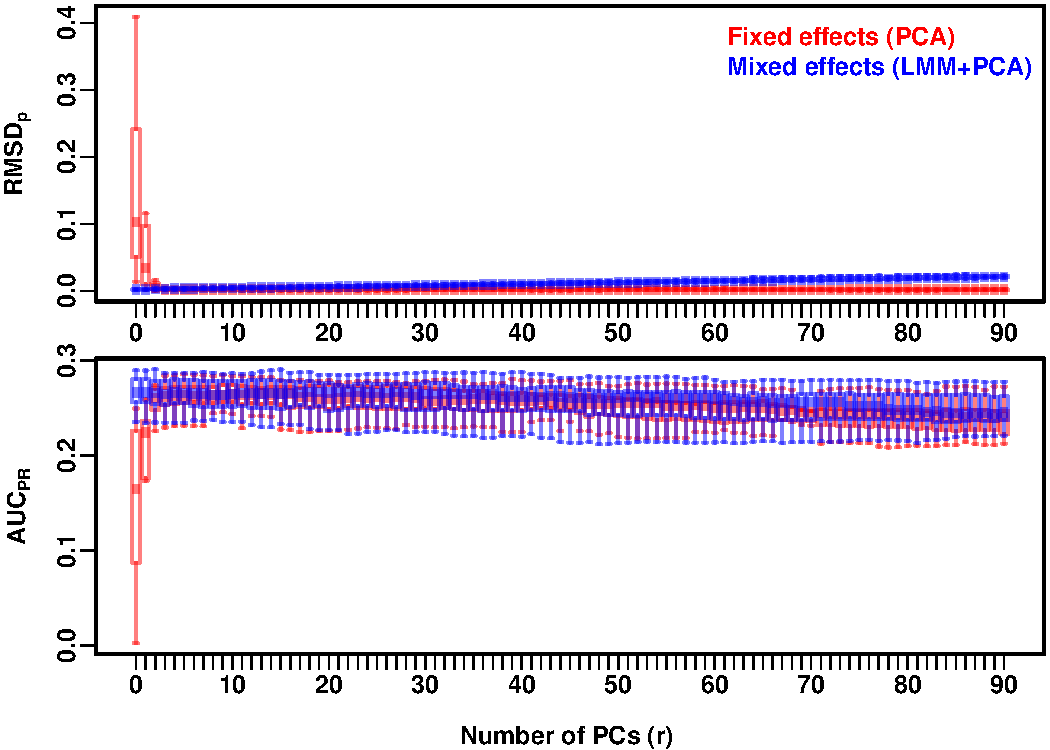
\includegraphics[width=6in]{PCA_data/PCA_GCTApcs/boxplot_n_1000.pdf}
  \caption{
    {\bf Evaluation in large sample size admixture scenario.}
    Here there are $n = 1,000$ individuals in the simulation.
    The PCA and LMM approach are tested under varying number of PCs ($r \in \{0, ..., 90\}$ on x-axis), with boxplots for 10 replicates (y-axis) for the distributions of $\rmsd$ (top panel) and $\auc$ (bottom panel).
    Small $\rmsd$ and large $\auc$ correspond with better performance.
    For mixed effects (LMM), the optimal number of PCs is $r=0$ since $\rmsd$ increases and $\auc$ decreases with increasing $r$.
    For fixed effects only (PCA), the ideal number of PCs is $r = 9$ in theory for PCA approach, but optimal performance is achieved with as few as $r = 4$ PCs, which results in near zero $\rmsd$ and peak $\auc$, and performs as well as the LMM without PCs.
    PCA with $r < 3$ has incorrect p-values ($\rmsd \gg 0$ cases) and lowest predictive power (small $\auc$).
    Remarkably, PCA is robust in extreme $r \gg 9$ cases, with $\rmsd$ near zero up to $r = 90$ and minimal loss of power as $r$ increases to 90.
  }
  \label{fig:large_sample_size}
\end{figure}

First we evaluate all methods in the large sample size scenario without close relatives, which has a reasonable number of individuals ($n = 1,000$) typical for genetic association studies.

We being by discussing the performance of the fixed effects model (PCA) as the number of PCs is varied.
In this scenario we find a clear transition around $r = 4$ number of PCs for PCA, below of which performance is poor and above of which performance is satisfactory (\cref{fig:large_sample_size}).
In particular, when $r < 3$ we find the largest $\rmsd$ values, which indicate that p-values are highly non-uniform and would therefore result in inaccurate type-I error control.
The smallest $\auc$ values also occur for $r < 3$, showing that not enough PCs results in loss of predictive power as well.
Interestingly, performance is optimal when the number of PCs is lower than the ideal value of $r=9$ according to theory (it is not necessary to model all of the 10 ancestries, modeling the most divergent 5 dimensions suffices).
%As expected, $r = 2$ has the best performance in terms of both $\rmsd$ and $\auc$.
Remarkably, as $r$ is increased up to $r = 90$, there is no noticeable change in the $\rmsd$ distribution, and only a small decrease in $\auc$ compared to the optimal $r = 4$ case.
Accurate null p-values under excessive numbers of PCs makes sense since the exact F-test is being used, whose performance is not affected by having too many covariates.

Now we turn to the mixed effects model (LMM), which models structure as a random effect and is tested here in combination with varying numbers of PCs used as fixed effect covariates.
The LMM without PCs ($r=0$) performs as well as PCA with $r = 4$, with small $\rmsd$ values and a slightly larger $\auc$ values than PCA with $r = 4$.
The performance of LMM worsens monotonically as $r$ increases.
The decreasing $\auc$ of LMM as $r$ increases tracks closely with the decreasing $\auc$ of the fixed-effects model only, suggesting that overfitting due to including too many covariates is causing the decrease in $\auc$.
Interestingly, $\rmsd$ increases for LMM as $r$ increases, an effect that was not observed for fixed effects only.
As we will cover in greater depth in the discussion, this is due to LMMs evaluating significance using asymptotic tests such as the likelihood ratio test, which become less accurate as the number of covariates increases, whereas our fixed effects null statistics are calculated with the F-test that is accurate for all values of $r$.

Overall, in this common scenario where sample sizes are large enough and there is no family structure, the LMM approach without PCs performs best, but the (fixed effects only) PCA approach performs as well as LMM as long as enough PCs are used.

\subsection{Small sample size simulation}

\begin{figure}[bp!]
  \centering
  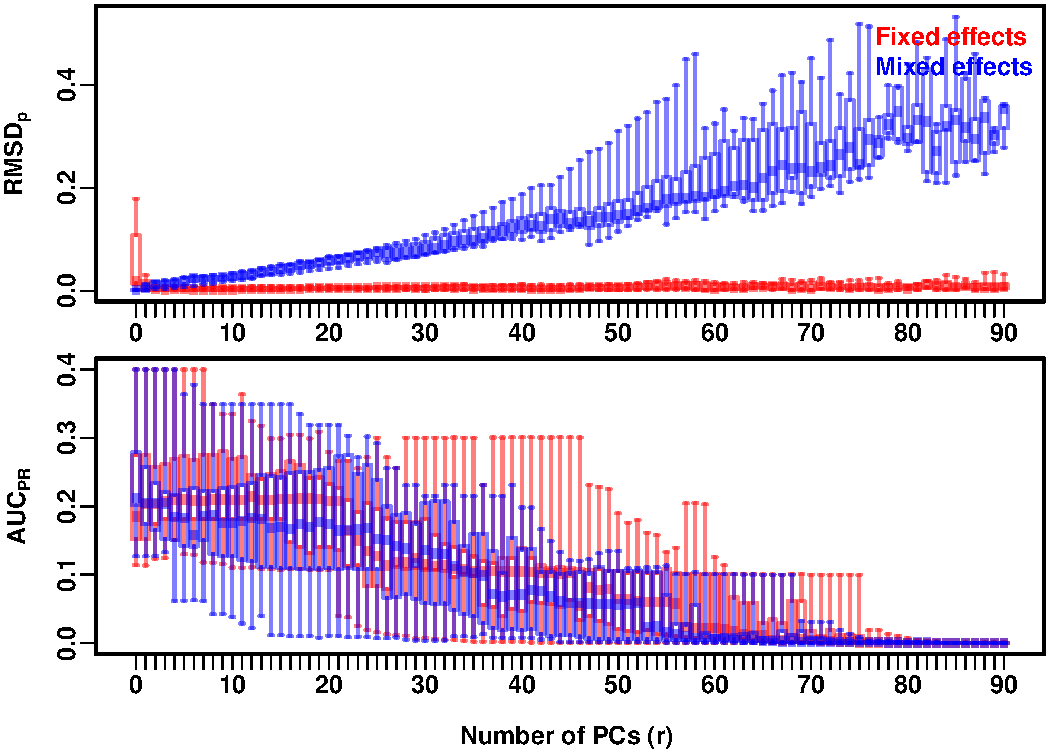
\includegraphics[width=6in]{PCA_data/PCA_GCTApcs/boxplot_n_100.pdf}
  \caption{
    {\bf Evaluation in small sample size admixture scenario.}
    Here there are $n = 100$ individuals in the simulation, otherwise the simulation and figure layout is the same as in \cref{fig:large_sample_size}.
    For fixed effects, the pattern for $\rmsd$ is similar to the previous figure, while $\auc$ drops faster as the number of PCs $r$ increases from $r=2$ to $r=90$.
    For mixed effects, the $\auc$ pattern mirrors that of fixed effects, whereas the $\rmsd$ increases with $r$ much faster here than in the previous large sample size simulation (the asymptotic $\chi^2$ approximation fails under small sample sizes and large numbers of covariates).
  }
  \label{fig:small_sample_size}
\end{figure}

In the previous case PCA performed well when the number of PCs was orders of magnitude greater than its ideal value in theory ($r = 90$ vs $r = 9$), which motivated us to find scenarios where this is no longer the case.
We expect the PCA approach to overfit more severely as the number of PCs $r$ approaches the sample size $n$.
Increasing $r$ beyond 90 would never be done in practice; 
instead, we reduced the number of individuals $n$ to 100, which is small for typical association studies, but which may occur in studies of rare diseases, or be due to low budgets or other constraints.
To compensate for the loss of power that results from reducing the sample size, we also reduced the number of causal loci from 100 before to $m_1 = 10$, which increases the magnitude of the effect sizes.
Note that this reduction in the number of causal loci results in more discreteness in $\auc$ values in \cref{fig:small_sample_size}.

We find that the relationship between $\rmsd$ and $r$ the same under small and large sample sizes for PCA (fixed effects), with ideal near-zero $\rmsd$ distributions for $r \ge 2$.
On the other hand, we see a more severe overfitting effect here that results in decreased predictive power: $\auc$ peaks at $r = 4$, then drops rapidly as $r$ increases, with performance around $r = 25$ that is worse than for $r = 0$, and practically zero $\auc$ at $r = 90$ (\cref{fig:small_sample_size}).
Thus, the overfitting effect is quite dramatic in studies with few individuals, where choosing the correct number of PCs is very important.

The behavior of LMM (mixed effects) with varying numbers of PCs is a more extreme version than what we observed in the large sample size simulation.
The mixed effects model performs increasingly poorly as $r$ increases ($\rmsd$ increases and $\auc$ decreases).
Just as in the first simulation, here the optimal choice is to use LMM without PCs, which successfully avoids overfitting and outperforms the best-performing fixed-effects method with $r=4$ PCs.



\subsection{Family structure admixture simulation}

\begin{figure}[bp!]
  \centering
  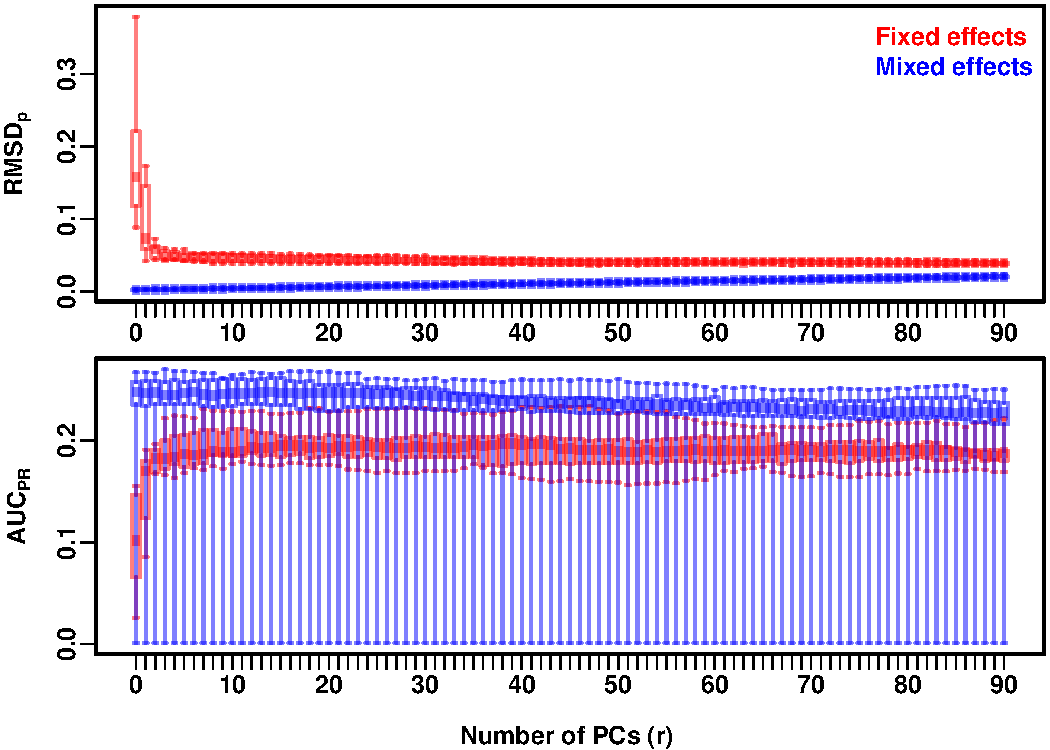
\includegraphics[width=6in]{PCA_data/PCA_GCTApcs/boxplot_n_1000_family.pdf}
  \caption{
    {\bf Evaluation in family structure admixture scenario.}
    Here there are $n = 1,000$ individuals from a family structure simulation with admixed founders and large numbers of pairs of sibling, first cousins, second cousins, etc, from a realistic random pedigree that spans 20 generations.
    Unlike previous figures, here fixed effects never perform as well as LMM, since $\rmsd$ (top panel) does not go down to zero as $r$ increases, and there is a significant gap in $\auc$ performance, as expected because of the presence of family structure.
    The LMM achieves a near-zero $\rmsd$ and the highest $\auc$ when no PCs are used ($r=0$).
  }
  \label{fig:family_structure}
\end{figure}

Previous work has shown that PCA performs poorly in the presence of family structure.
Here we aim to characterize PCA's behavior in a much more complex structure than before, by simulating a family of admixed founders for 20 generations, so that we may observe numerous siblings, first cousins, etc, while mostly preserving the population structure due to ancestry by biasing pairings for more similar ancestries.

In this case PCA improves in performance until around $r \approx 15$, which is larger since the family structure increases the rank of the genotype matrix compared to the previous simulations without family structure.
We find that, although $\rmsd$ for PCA decreases monotonically as $r$ increases, this distribution does not go to zero, instead converging to around 0.05 (\cref{fig:family_structure}).
In contrast, for mixed effects, $\rmsd$ is practically zero at $r=0$, but $\rmsd$ increases with increasing $r$ (similar to the pattern for large sample sizes without family structure in \cref{fig:large_sample_size}).
In terms of $\auc$, fixed effects has its best performance at $r=15$, but
A sizable gap in $\auc$ performance is observed for PCA compared to LMM with $r = 0$, which performs best.
Overall, LMM conclusively outperforms PCA (fixed effects only) in the case of family structure. 

\section{Discussion}

% \citep{zhang_semiparametric_2003}:
% First PCA application to GWAS, for quantitative traits, albeit a more complicated implementation than is more common now in practice.
% Measures type-I error and power.
% SIM: IS and admixture, $K = 2$, extremely small sample sizes ($m = 300$, $n = 150$).
% Tested $r = 1$ only.

% \citep{price_principal_2006}:
% case-control
% sim: $n = 1000$, $m = 100,000$, IS $K = 2$, admixture .
% Data analysis: $n = 488$, $m = 116,204$.
% Tested PCA with $r = 1, 2, 5, 10$.
% They find that $m > 20,000$ is needed for PCA to work reliably (depends on \Fst).

% \citep{patterson_population_2006}:
% The statistical method for picking $r$ (Tracy-Widom?).

% \citep{yu_unified_2006}:
% PCA vs LMM, LMM is based on kinship estimates from pedigree or genotypes (a la Ritland), plus admixture proportions Q from STRUCTURE.
% So not exactly a PCA comparison.
% Measure both p-value uniformity (visually) and power only for a few genes' expression as phenotypes.

% \citep{epstein_simple_2007}:
% case-control.
% Shows PCA doesn't work with $r=10$, seems to fall under small sample size scenario!
% No LMM.
% Introduces a new statistical approach for this.
% Measures type-I error and power.

% \citep{kimmel_randomization_2007}:
% They're supposed to show cases where eigenstrat is not so good!
% Tests PCA (mentions LMM but does not test), don't clarify which $r$ was used.
% Introduces randomization approach ``PSAT'', says they get an LD advantage.
% Therefore, expect PCA to approach PSAT performance when LD is zero.
% Case-control.
% Measured type-I error and power.
% HapMap-based simulation, Li-Stephens style.

% \citep{zhao_arabidopsis_2007}:
% LMM vs PCA and others in arabidopsis.
% Did not vary number of PCs (used $r = 8$).
% Looks at p-value uniformity (visually), but potentially included non-null loci in figures.
% Looks at power too, averaged over a few simulations.

% \citep{luca_use_2008}.
% Introduces genetic control matching.
% Measure type-1 error and power.
% sim: IS and admixture $K=2$, all small sample sizes ($n = 400$, $m = 24,000$).
% What was $D$ (our $r$) set to in examples?
% PCA flaws pointed out: small sample sizes, outliers.

% \citep{zhang_comparison_2008}:
% PCA most robust, comparable to SA.
% PCA $r$ value used not clarified!
% LMMs not evaluated.
% sims: hapmap-based, case-control only.
% measure type-1 error and power.

% \citep{li_improved_2008}:
% Case-control, sim IS and admixture.
% PCA ($r = 10$) and other related approaches, no LMM.
% Introduces MDS?  Also has clustering as second set of covariates.
% MDS outperforms eigenstrat, is that weird?

% \citep{kang_efficient_2008}:
% no PCA comparison, but yes SA.
% p-values included SA.
% Power was for EMMA only, various simulated traits.

% \citep{astle_population_2009}:
% sim case-control $n = 2000$, $m = 10,000$, IS $K = 3$.
% Tested PCA with $r = 10$.
% Measures p-value uniformity and ROC curves.
% PCA and LMMs are tied in this setting, like our large sample size scenario!
% LMM appears slightly better than PCA under case/control ascertainment bias.

% \citep{li_correcting_2010}:
% Introduces ``phylostrat''.
% PCA $r = 10$ tested only, also compared to MDS and related stuff; No LMM.
% As before, case-control and sim IS and admixture.
% Measured type-I error and power.

% \citep{kang_variance_2010}:
% EMMAX, compares to eigenstrat with $r = 100$!
% Does vary $r$ somewhat, its Fig. 2 shows little improvement after $r \ge 5$ for most traits.
% Looks at GC inflation factor.
% No power evaluations!

% \citep{price_new_2010}:
% Compares PCA $r=1$ and LMM using lambda only.
% Simplistic simulations with $K=2$ independent subpops or simple siblings(?)
% Suggests LMM+PCA is best of both worlds.

% \citep{wu_comparison_2011}:
% case control only, ``unrelated'' samples! (deletes LMM advantage).
% $r = 10$ only.
% sims: discrete subpops and admixture ($K=2$; again, no fams).
% evaluate using p-values and power.
% Conclusion is PCA et al are better for SNPs under selection or high differentiation.

% \citep{bouaziz_accounting_2011}:
% Yes PCA $r=5$, but no LMMs?
% case control only?
% Sims: HapMap-based and admixture (simple).

% \citep{hoffman_correcting_2013}:
% Simulates confounding directly from PCs! (BAD)
% Measures power mostly.
% One p-value figure.
% Doesn't discuss pure PCA much, in some cases PCA seems to outperform vanilla LMM!

% \citep{sul_mixed_2013}:
% Counters that random effects are not by themselves inferior to fixed effects.
% Shows a more complex LMM fits the weird ``selection'' simulation just as well.
% Also only lambda (like Price).

% \citep{price_response_2013}:
% A boring acknowledgment, no new tests or conclusions really.

% \citep{wang_analytical_2013}:
% Compares PCA and LMM!
% Weird argument places non-family structure entirely in the intercept, but with individual-specific values.
% Also LMMs are modeled through their BLUE estimates and not REML as in practice, evals use this unsual model too.
% They look at t-statistics (like p-value uniformity), no direct power measurement.
% Sim: rho relatedness, and IS with $K = 4$.

% \citep{tucker_improving_2014}:
% PC select, a sparse version to rival Fast-LMM.
% Tested $r = 5$ only.
% Sim: $n = 1000$, $m = 10,000$, other details unclear.
% Measure inflation and power.

% \citep{yang_advantages_2014}:
% Mostly LMMs, they say they test PCA with $r=5$.
% Evaluation is only on real data, no type-I error or power.

% \citep{sul_population_2018}:
% LMM review.
% They show lambdas for real datasets, comparing EMMAX to PCA with $r = 100$.
% LMM better than PCA, is it because of cryptic relatives?

% \citep{wojcik_genetic_2019}:
% Modern example with PCA $r = 10$ and a method that determines that this is a good choice (tested $r = 1, ..., 10$).

Our main findings are organized into three areas:
(1) the robustness of the performance of PCA (fixed effects only) on the number of PCs included;
(2) the performance of LMM (mixed effects) when PCs are included; and
(3) the overall comparison between LMM and PCA.
In each case we will discuss how performance depended on various aspects of each simulation.

\subsection{Robustness of PCA (fixed effects only) to the number of PCs}

One important conclusion of our evaluation is that the PCA approach for genetic association studies (fixed effects only) is robust to the choice of $r$ (number of PCs), as long as $r$ is large enough, especially when the sample size is large enough.
Thus, while we expect an $r$ that is too small or too large may hurt the performance of PCA (by not modeling enough of the population structure, or by overfitting, respectively), we find that the magnitude of the performance penalty depends very strongly on whether $r$ is too small or too large.

In our simulations that excluded family structure, the optimal choice for PCA (fixed effects only) was $r \approx 4$, which was smaller than the theoretical optimal value of $r=9$ when we consider the number of ancestries ($K=10$) and the intercept coefficient.
We found that insufficient PCs such as $r = 1$ paid a large penalty in both type-I error control (measured via $\rmsd$) and predictive power ($\auc$; \cref{fig:large_sample_size,fig:small_sample_size}).
In contrast, $r$ can be much larger than its optimal value with no penalty in terms of type-I error control (regardless of sample size), and only a negligible cost in predictive power when sample sizes are large (\cref{fig:large_sample_size}).
Successful type-I error control (\textit{i.e.}, near zero $\rmsd$) for fixed effects and for large enough numbers of PCs ($r$) follow from our use of the F-test for calculating statistical significance, which holds exactly for all $r$ values and does not rely on asymptotic approximations.
The loss of predictive power by using excessive PCs is only pronounced when the number of individuals $n$ is much smaller than is common nowadays, \textit{i.e.}, in the hundreds (\cref{fig:small_sample_size}).
This robustness of PCA to the choice of $r$ has long been anecdotal only \citep{price_principal_2006, kang_variance_2010}.
Here we conclusively found that it is far safer to err on the side of larger $r$, especially for large sample sizes, although testing several $r$ values via simulations is always recommended.

The presence of family structure is the main weakness of the PCA approach.
Type-I error is never accurately controlled ($\rmsd$ was non-zero) for any number of PCs we tested (up to $r=90$; \cref{fig:family_structure}).
The pattern of $\auc$ here resembles that of the simulation without family structure (except optimal performance is achieved around $r = 15$), but best performance is never as good as for LMMs.

\subsection{Robustness of LMM (mixed effects) to the number of PCs}

We also evaluated use of an LMM (Linear Mixed-effects Model) in combination with PCs, an approach that has performed best in certain previous evaluations \citep{zhao_arabidopsis_2007, price_new_2010}.
In all of our simulations we found that LMM with zero PCs always outperformed using any non-zero number of PCs \cref{fig:large_sample_size,fig:small_sample_size,fig:family_structure}).
Our findings make sense since the eigenvectors of the kinship matrix (used as the covariance of the random effects) are the same as the PCs in the PCA approach, so including both is redundant.
It is possible that there are more complex scenarios than considered here where an LMM with PCs performs better than LMM without PCs.

Although our evaluations favor using LMM without PCs, our tests also revealed that LMMs with large numbers of covariates suffer from inaccurate p-values, an LMM-specific problem that we did not observe for fixed effects.
The key difference between the two approaches is that p-values for fixed effects are calculated from an exact distribution (F-test), which is robust to large numbers of covariates, while mixed effects necessitate an approximatimation (the likelihood ratio test has test statistics which are only are asymptotically $\chi^2$).
These approximations become more unreliable the more covariates are present, as observed in our evaluations.
Unfortunately, there is no alternative to the likelihood ratio test in LMMs.
Again, LMM with zero PCs is the best performing method and in that case p-values are accurate.
However, the same issue of problematic statistics can arise where a large number of (non-PC) covariates are being fit in an association study, particularly when the number of individuals is small, as in our small sample size simulation (\cref{fig:small_sample_size}).

\subsection{Overall comparison between LMM and PCA}

Previous work has mostly ruled in favor of LMM (mixed effects) versus PCA (fixed effects only), or otherwise tend to show comparable performance.
Our simulations agree that LMM is always the best choice, but the gap in performance of PCA (with the optimal choice of numbers of PCs) varies depending on the simulation.
The clearest theoretical advantage of the LMM is its ability to model family relatedness.
We confirm this in our family structure simulation, where LMM (without PCs) significantly outperforms the best PCA model in terms of both type-I error control ($\rmsd$) and predictive performance ($\auc$; \cref{fig:family_structure}).
The other theoretical advantage of LMM over PCA is in having fewer degrees of freedom \citep{hoffman_correcting_2013}; however, we did not see this improving $\auc$ in our small sample size simulation where overfitting overall played a large role: the best PCA model performed as well as LMM (\cref{fig:small_sample_size}).
However, PCA can perform poorly when the number of PCs is not chosen carefully, especially under small sample sizes, which may explain early claims that PCA was not effective in preventing test statistic inflation \citep{epstein_simple_2007, kimmel_randomization_2007, luca_use_2008}.

Evaluations from others suggest that PCA can outperform LMM when there are loci under selection or otherwise highly differentiated, and rare variants \citep{price_new_2010, wu_comparison_2011, yang_advantages_2014}.
One potential explanation is that the additional degrees of freedom in the additional PCs enables the LMM to better model loci when the pure ($r=0$) LMM model assumptions break.
However, our simulations indicate that LMM is the best choice for most population structures.
Since PCA matches the performance of LMM when there is no family structure, this argues against the simple characterization that either fixed or random effects are in principle superior models for association studies \citep{price_new_2010, sul_mixed_2013, price_response_2013, sul_population_2018}.
The driving principle that explains the PCA and LMM performance is the dimensionality of the genetic structure:
when there is no family structure, then structure is low dimensional, so either PCA and LMM are well suited for modeling the population structure.
In contrast, the presence of family relationships increases the dimensionality of the genetic structure, and in that case PCA performs poorly because either not enough PCs are used, or instead so many PCs are needed that overfitting occurs.
LMMs naturally model pedigrees via kinship matrices, and in general they fit arbitrary high-dimensional genetic structures, and having fewer effective parameters than PCA prevents overfitting of the data.

In addition to our findings, another advantage of LMMs is that the user need not choose parameters arbitrarily, as is sometimes the case for the number of PCs in the PCA approach.
Thus, the key practical advantage of PCA is its speed, as fitting mixed-effects models has a higher computational complexity.
However, modern LMM implementations are much faster than the first generation of LMMs for genetic association.
Moreover, if the number of PCs to use is not known, then expensive simulations need to be performed to determine this number, and this may also eliminate the computational advantage of running PCA compared to LMM.
For these reasons, we recommend always using LMMs when it is computationally feasible.
On the other hand, it is important to understand whether use of PCA in past association studies has resulted in a relative increase of false positives or false negatives.
Our simulations suggest that PCA results in accurate association studies as long as
(1) there are no close relatives present in the study,
(2) enough PCs were used, and
(3) sample sizes are large enough.
Common practice of large sample sizes, excluding close relatives, and using at least 10 PCs suggests that the majority of previous genetic association studies that used PCA have presented valid results on par with what an LMM would have reported.

\printbibliography



\end{document}